
\documentclass[conference]{IEEEtran}

\hyphenation{op-tical net-works semi-conduc-tor}


\usepackage[portuguese]{babel}
\usepackage[utf8]{inputenc}		% Codificacao do documento (conversão automática dos acentos)

\usepackage{rotating}
\usepackage{tabularx}
\usepackage{multicol}
\usepackage{amsmath}
\usepackage[linesnumbered,ruled]{algorithm2e}

\usepackage{caption}
\usepackage{subcaption}

% Define o caminho das figuras
\graphicspath{{images/}}


\begin{document}
\title{Segmentação Textual Automática de Atas de Reunião}


%\author{
%\IEEEauthorblockN{Ovídio José Francisco}
%\IEEEauthorblockA{UFSCar -- Sorocaba\\
%Email: ovidiojf@gmail.com}
%}

\newcommand{\urlatas}{http://www.ppgccs.net/?page\_id=1150}
\newcommand{\urlbrowcorpus}{http://clu.uni.no/icame/brown/bcm.html}
\newcommand{\urlreuterscorpus}{http://trec.nist.gov/data/reuters/reuters.html}
\newcommand{\urlicsi}{http://www1.icsi.berkeley.edu/Speech/mr}



\maketitle


\IEEEpeerreviewmaketitle



	\begin{resumo}
%
% Breve defini��o de segmenta��o
%%%
A tarefa de segmenta��o textual consiste em dividir um texto em por��es com significado relativamente independente, de maneira que cada segmento contenha um assunto. 
%
% Literatura focada em documentos longos
%%%
Muitas pesquisas avaliam t�cnicas de segmenta��o textual usando textos longos com a concatena��o de not�cias de v�rios assuntos ou com a transcri��o de discursos ou reuni�es com m�ltiplos participantes.  
%
% Maior foco e perfomance no ingl�s
%%%
%Al�m disso, a maior parte das pesquisas � realizada considerando o idioma ingl�s.
%
% Peculiaridades das atas
%%%
%Esse artigo tem como objeto de estudo atas de reuni�o escritas em portugu�s, as quais as al�m do idioma menos estudado sob essas t�cnicas, possuem estilo de reda��o mais formal e sucinto.
%, o que desfavorece t�cnicas baseadas em frequ�ncia de palavras. 
%
% Utilidade
%%%
%A segmenta��o desses documentos facilita a sua organiza��o e acesso, oferecendo vantagens no processo de recupera��o de informa��o em rela��o � busca por palavras-chave, pois � poss�vel retornar por��es de texto menores que contenham assuntos relevantes � inten��o do usu�rio, ao inv�s de destacar as palavras-chave em um texto longo que pode conter informa��es menos pertinentes. 
%
% Objetivo: Adaptar algs e encontar melhor t�cnica
%%%
%
%
Este artigo concentra-se nos principais algoritmos da literatura aplicando-os 
%
%um conjunto de atas do departamento de p�s-gradua��o da UFSCar-Sorocaba foi manualmente segmentado por participantes das reuni�es
%
ao contexto das atas de reuni�o em portugu�s, 
%
as quais as al�m do idioma menos estudado com essas t�cnicas, possuem estilo de reda��o mais formal e sucinto. 
%
%
Ao final, chegou-se a uma t�cnica capaz de segmentar as atas com performance similar a outros trabalhos da literatura. 



% e visa encontrar uma t�cnica que ofere�a segmentos coesos e contribua para aprimorar sistemas de recupera��o de informa��o para que respondam melhor � buscas do usu�rio.


%
% Configura��o melhor avaliada
%%%
% Para a avalia��o experimental, um conjunto de atas do departamento de p�s-gradua��o da UFSCar-Sorocaba foi manualmente segmentado por participantes das reuni�es. Ent�o, as divis�es manuais foram comparadas com as divis�es geradas automaticamente a fim de encontrar uma configura��o que melhor retorne segmentos coesos de atas de reuni�o. Ao final, chegou-se a uma t�cnica capaz de segmentar as atas com performance similar a outros trabalhos da literatura. 
%
%
\end{resumo}

\begin{abstract}
The abstract goes here!
\end{abstract}
	





% As atas de reuni�o possuem estilo de reda��o mais formal e sucinto, o que desfavorece t�cnicas baseadas em frequ�ncia de palavras.

% Por conta disso, muitos segmentadores apresentam melhor performance nessas condi��es.

% Sumariza��o  ??????
% Etapa de pre-processamento ???
%apresenta vantagens em rela��o a organiza��o manual 

%frequentemente s�o escritas em par�grafo �nico  e n�o apresentam marca��es de estrutura como cap�tulos ou se��es. Al�m disso, 

% Al�m disso, a segmenta��o de textos longos pode aprimorar a navega��o pelo documento, sobre tudo por usu�rios com defici�ncia visual.

% entregando segmentos com significado relativamente independente do documento. 

% se levado em conta a peculiaridade desses documentos.

%Os testes registraram precis�o de 0.7106, revoca��o de 0.8516, as medidas P$_k$ e \textit{WindowDiff} mostram respectivamente 0.1163 e 0.3800 de dissimilaridade.

% na adapta��o dos algoritmos mais influentes ao contexto das atas de 

%a fim de melhor responder a buscas do usu�rio em sistemas de recupera��o de informa��o.

%divida um documento em partes .



% os influentes tratam muito de discursos e textos longos
% as atas apresentam texto mais enxuto/compacto e com estilo pr�prio.
% as atas s�o uma par�frase da reuni�o


	Frequentemente atas de reunião tem a característica de apresentar um texto com poucas quebras de parágrafo e sem marcações de estrutura, como capítulos, seções ou quaisquer indicações sobre o tema do texto. 


% Definição 

A tarefa de segmentação textual consiste dividir um texto em partes que contenham um significado relativamente independente. Em outras palavras, é identificar as posições onde há uma mudança significativa de tópicos.

% Usos
É útil em aplicações que trabalham com textos sem quebras de assunto, ou seja, não apresentam parágrafos, seções ou capítulos, como transcrições automáticas de áudio e grandes documentos que contêm assuntos não idênticos como atas de reunião e noticias.


% Interesses
O interesse por segmentação textual tem crescido em em aplicações voltadas a recuperação de informação %citar o [15] ...
e sumarização de textos. % ... e [2] do "Efficient Linear T S"
Essa técnica pode ser usada para aprimorar o acessao a informação quando essa é solicitada por um usário por meio de uma consulta, onde é possível oferecer porções menores de texto mais relevante ao invés de exibir um documento maior que pode conter informações menos pertinente. A sumarização de texto também pode ser aprimorada ao processar segmentos separados por tópicos ao invés de documentos inteiros.


% Coesão Léxica
Os algoritmos avaliados baseiam-se na ideia de coesão léxica entre assuntos. Isto é, a mudança de tópicos é acompanhada % é relacionada à
 de uma proporcional mudança de vocabulário. A partir disso, vários algorítmos foram propostos. Nesse artigo, os principais serão analizados na prespectiva de atas de reunião.





% Diversas aplicações fazem uso de segmentação textual, incluindo 

% Entre as principais mais frequentes de segmentação textual estão a tra



%É principalmente utilizada em aplicações que processam textos longos como transcrições de áudio e documentos longos, além de aprimorar técnicas de sumarização e information retrievel.



% Usos:
%	* quando não há identificações
%	* em transcrições de áudio
%	* em documentos longos
% 	* text summarization (ver a referencia [2] de Efficient Linear Text...)




%Isto é, dado um texto, identificar onde há mudança de tópicos.


% Interest in automatic text segmentation has blossomed over the last few years, with applications ranging from information retrieval to text summariza-tion to story segmentation of video feeds. [A Critique and Improvement of an Evaluation Metric for Text Segmentation]



%Em outras palavras é identificar divisões entre unidade de informação sucessivas

%A tarefa de segmentação textual consiste em encontrar pontos onde há mudança de tópicos no texto.



%[ The task of linear text segmentation is to split a large text document into shorter fragments, usually blocks of consecutive sentences. ]


% **Segmentação é identificar divisiões entre unidades de informação sucessivas (Beeferman, Berger, and Lafferty (1997))**

%   [Text segmentation is the task of determining the positions at which topics change in a stream of text]





	\section{Referencial Teórico}
	\label{referencial}
	
%%%%%%%%%%
% Retomada das Definições
%%%%%%%%%%	

Um documento textual, sobre tudo quando longos, são frequentemente um sucessão de tópicos. 

%%%%%%%%%%
% Segmentação
%%%%%%%%%%
Segmentação topical ou segmentação linear é a tarefa de dividir um texto em partes mantendo nas partes o texto de um tópico com seu significado completo.
	
%%%%%%%%%%
% Segmento
%%%%%%%%%%	
Um segmento pode ser visto como uma sucessão de unidades de informação que compartilham um tópico e podem ser, por exemplo, palavras, sentenças ou parágrafos. Essas unidades são a menor parte de um segmento e portanto consideradas candidatas a limite entre segmentos, bem como é necessário mensurar suas similaridades.

%%%%%%%%%%
% Coesão léxica como **presuposto básico**
%%%%%%%%%%
Trabalhos anteriores apontam que a coesão léxica é um forte indicador da estrutura do texto~\cite{Galley2003}~\cite{Boguraev2000}.
%Os principais algoritmos de segmentação textual baseiam-se na ideia de coesão léxica em um assunto.
Isto é, a mudança de tópicos é acompanhada de uma proporcional mudança de vocabulário. A partir disso, vários algoritmos foram propostos baseados na ideia de que um segmento pode ser identificado e delimitado pela análise das palavras que o compõe.



%%%%%%%%%%
% Porque cosseno
%%%%%%%%%%
Uma vez que a coesão léxica é pressuposto básico da maioria dos algoritmos, o cálculo da similaridade entre textos e fundamental. Uma medida de similidade frequentemente utilizada é o cosseno, o qual pode ser vista na Equação~\ref{equ:cosine}, sendo $f_{x,j}$ a frequência da palavra $j$ na sentença $x$ e $f_{y,j}$ sendo a frequência da palavra $j$ na sentença $y$.


\begin{equation}
Sim(x,y) = \frac
{\Sigma_j f_{x,j} \times f_{y,j}}
{\sqrt{\Sigma_j f^2_{x,j} \times \Sigma f^2_{x,j}}}
\label{equ:cosine}
\end{equation}


%%%%%%%%%%%%%%%%%%%%%%%%%%%%%%%%%%%%%%%%%%%%%%%
%%%              TextTiling                 %%%
%%%%%%%%%%%%%%%%%%%%%%%%%%%%%%%%%%%%%%%%%%%%%%%

Entre os trabalhos mais influentes podemos citar o \textit{TextTiling}~\cite{Hearst1994} proposto por Hearst. Ela propõe um algoritmo baseado em janelas deslizantes, onde para cada candidato a limite, analisa-se o texto circundante. Um limite ou quebra de segmento é identificado quando a similaridade entres os blocos apresenta uma queda considerável.

%Ela propõe um algoritmo baseado em janelas deslizante, para analisar blocos de texto adjacentes e identificar os limites com base nas similaridades dos blocos.

O algoritmo recebe uma lista de candidatos a limite, usualmente finais de parágrafo ou finais de sentenças. Para cada posição candidata são construídos 2 blocos, um contendo sentenças que a precedem e outro com as que a sucedem. O tamanho desses blocos é um parâmetro a ser fornecido ao algoritmo e determina o tamanho mínimo de um segmento.
%
Em seguida, os blocos de texto são representados por vetores que contém as frequências de suas palavras. Então, usa-se cosseno (Equação~\ref{equ:cosine}) para calcular a similaridade entre os blocos.

Finalmente, os limites são identificados sempre que a similaridade entre blocos adjacentes entre cada candidato ultrapassa um determinado \textit{threshold}.

O \textit{TextTiling} apresenta baixa complexidade computacional, devido a simplicidade do algoritmo e baixa eficiência quando comparado a outros métodos mais sofisticados como mostrando em~\cite{Choi2000, Kern2009}.



%%%%%%%%%%%%%%%%%%%%%%%%%%%%%%%%%%%%%%%%%%%%%%%
%%%                  C99                    %%%
%%%%%%%%%%%%%%%%%%%%%%%%%%%%%%%%%%%%%%%%%%%%%%%

Choi \cite{Choi2000} apresenta um esquema de ranking em seu algoritmo, o \textit{C99}. 
%
Embora muitos trabalhos utilizem matrizes de similaridades, o autor traz obervações.
%
Ele aponta que para pequenos segmentos, o cálculo de suas similaridades não é confiável. Pois uma ocorrência adicional de uma palavra causa um impacto desproporcional no cálculo.
%
Além disso, o estilo da escrita pode não ser constante em todo o texto. Choi sugere que, por exemplo, textos iniciais dedicados a introdução costumam apresentar menor coesão do que trechos dedicados a um tópico específico. 
%

Portanto comparar a similaridade entre trechos de diferentes regiões, não é apropriado.
% Complexidade O(n²)
Devido a isso, as similaridades não podem ser comparadas em valores absolutos,  então, o autor apresenta um esquema de \textit{ranking} para contornar esse problema.
%



Cada valor na matriz de similaridade é substituído por seu ranking local. Onde \textit{ranking} é o número de elementos vizinhos com similaridade menor, o qual é calculado com a Equação~\ref{equ:ranklocal}. Um exemplo é mostrado na Figura \ref{fig:exemplomatrixrank} abaixo, onde utiliza-se uma máscara de largura igual a 3.



  \begin{figure}[!h]

	\centering
	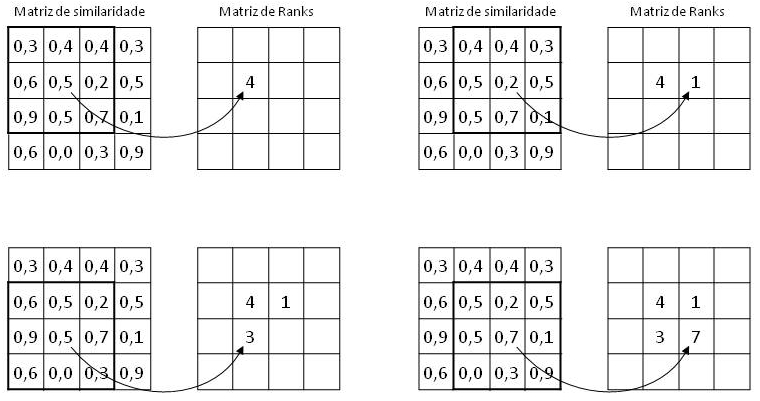
\includegraphics[width=0.45\textwidth]{exemplo-matrix-rank-noborder.jpg}
	\caption{Exemplo de construção de uma matriz de rank}
	\label{fig:exemplomatrixrank}

  \end{figure}




\begin{equation}
r(x,y) = \frac
{Numero\ de\ elementos\ com\ similaridade\ menor}
{Numero\ de\ elementos\ examinados}
\label{equ:ranklocal}
\end{equation}


% Clustering Reynar maximization
	
Finalmente, utiliza um método de divisão por \textit{clustering} baseado no algoritmo de maximização de Reynar~\cite{Reynar1998} para identificar os limites entre os segmentos. Essa abordagem apresenta uma redução taxa de erros de 22\% para 10\%. Por outro lado, exige que a quantidade de segmentos seja conhecida.
Como melhoramento, Choi apresenta posteriormente uma versão em seu trabalho ~\cite{Choi2001-LSA} que utiliza \textit{Latent Semantic Analisys} (LSA) para calcular as similaridades ao invês de \textit{cosine}.




% Mensionar que existem duas abordagens principais - Baseada em coesão léxiam e em discursos [ver a pg 2 do Text Segmentation With Topic Moeling and Entity Coherence]




%Há ainda outros critérios para segmentação como a segmentação temática 

%outros tipos de abordagem
%	Segmentação funcional
%	Segementação temática
	
	\section{Trabalhos Relacionados}
	\label{sec:trabalhos}


Semelhante a esse trabalho, outras abordagens foram propostas como em~\cite{CHAIBI2014} onde os autores adaptam os \textit{TextTiling} e \textit{C99} ao idioma árabe. Apresentam os resultados de experimentos no qual avaliam a performance em jornais de diferentes países em árabe. As adaptações consistem basicamente na etapa de pré-processamento e apontam que diferenças no dialeto de cada pais devem ser consideradas no processo de segmentação e que a adaptação depende da escolha de um \textit{stemmer} adequado.

É recorrente a aplicação de segmentadores à reuniões com múltiplos participantes onde se estuda os discursos extraídos de reuniões, ou seja, o texto a ser segmentado é uma transcrição das falas dos participantes durante a reunião.
%
Banerjee~\cite{Banerjee2006} apresenta um segmentador baseado no  \textit{TextTiling} ao contexto das reuniões, com múltiplos participantes. Utiliza como \textit{corpus} a transcrição da fala dos participantes durante a reunião a qual foi conduzida por um mediador que propunha os tópicos e anotava o tempo onde os participantes mudavam o assunto. 
% outros exemplos são

Ainda no contexto de reuniões com múltiplos participantes, alguns elementos da fala são utilizados para encontrar melhores segmentos.
%
Bokaei~\cite{Bokaei2015}, traz um trabalho voltado à segmentação funcional do texto, que foca na atividade dos participantes, as quais categoriza em diálogos e monólogos e sugere que alguns comportamentos podem dar pistas de mudança de tópico, como quando um participante toma a palavra por um tempo prolongado. 
Galley~\cite{Galley2003} por sua vez considera de elementos como pausas, trocas de falantes e entonação para encontrar melhores segmentos.

Kern aponta em sua pesquisa~\cite{Kern2009} que algoritmos que apresentam melhor performance o fazem ao custo de maior complexidade computacional, que se deve à construção de matrizes de similaridade entre todas as sentenças como em~\cite{Choi2000}. Ele apresenta uma abordagem que otimiza o cálculo ao computar as médias das similaridades de cada bloco, a qual chama de \textit{inner similarity} e em seguida usa esses valores para calcular as medias das similaridades entre todos os blocos a qual chama de \textit{outter similarity}. Dessa forma não é criada uma matriz que contem as similaridades de todas as sentenças, mas apenas daquelas mais próximas. Os autores reportam uma eficiência superior e uma eficiência comparável aos algoritmos mais complexos.
% usa vetores contendo o peso da palavra ao inves da frequencia.



	\section{Proposta: Segmentação Linear Automática de Atas de Reunião}
	\label{sec:proposta}






%%%%%%%%%%
% TextTiling e C99 criados para inglês e independente de domínio
%%%%%%%%%%
Os algoritmos \textit{TextTiling} e \textit{C99} foram propostos para o inglês, independentemente de domínio, ou seja, a proposta inicial dos autores é trabalhar em qualquer texto nessa língua.
%%%%%%%%%%
% Adapatar para Atas em português
%%%%%%%%%%
Assim, propõe-se adaptá-los ao contexto das atas de reunião em português do Brasil, ou seja, em uma língua diferente e dentro de um contexto específico. As subseções seguintes tratam das adaptações para esse nicho mais específico. A Seção~\ref{sec:avaliacao} mostra a análise dos algoritmos adaptados.

%%%%%%%%%%
% Dificuldade: Coesão léxica não tão bem definida
%%%%%%%%%%
O vocabulário das reuniões, ainda que em tópicos diferentes, compartilham certo vocabulário pertencente ao ambiente onde se deram as reuniões. Isso é um fator que diminui a coesão léxica entre os segmentos.
%%%%%%%%%%
% Dificuldade: estilo da escrita
% - Paragrafo único
% - Cabeçalhos e rodapés
% - Pontuação --> ; encerrando sentenças
% - Insersão de espaços que não são quebra de sentença
% - Ruídos
%%%%%%%%%%
As atas de reunião costumam ter um estilo de escrita que deve ser levado em conta na adaptação do algoritmos, como a identificação de finais de sentença na ausência de quebras de parágrafo, inserção de linhas que não separam assuntos, utilização de pontuação para transição de tópicos, e cabeçalhos e numerais ruidosos. 

Nas subseções a seguir serão apresentados o pré-processamento e a identificação de segmentos candidatos considerados para a segmentação de atas.





\subsection{Pré-processamento}
	\label{subsec:preprocessamento}




	O texto a ser segmentado frequentemente é extraído de documentos em formatos como \textit{pdf}, \textit{doc}, \textit{docx} ou \textit{odt}. Após a extração do texto, esse pode passar por processos de transformação os quais serão apresentados a seguir.
	
%	A etapa de pré-processamento, em um documento contendo texto puro, acontece em quatro passos principais. 

  \begin{figure}[!h]
	\centering
	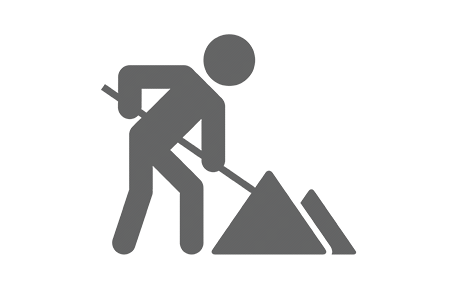
\includegraphics[width=0.2\textwidth]{construcao.png}
%	\caption{Exemplo de pré-processamento.}
	\\Em Construção
	\label{fig:exemplopreprocessamento}
  \end{figure}

	
%\begin{enumerate}


%
% 1) Identificação de sentenças
%\item \textit{Identificação de sentenças}: 
%Cada final de sentença e identificado e marcado com uma \textit{string} especial, esse processo é melhor descrito na Subseção~\ref{subsec:indentificacaosentencas}.
%
%conforme mostrado no Algoritmo~\ref{alg:identificacaofinaisdesent}.

%	
% 2) Eliminação de ruídos
%\item \textit{Remoção de ruídos}:

%%%%%%%%%%
% Cabeçalhos e rodapés
%%%%%%%%%%
%As atas frequentemente contém trechos que podem ser considerados pouco informativos e descartados durante o pré-processamento, como cabeçalhos e rodapés que se misturam aos tópicos tratados na reunião, podendo ser  inseridos no meio de um tópico e criando uma quebra que prejudica tanto o algoritmo de segmentação, quanto a leitura do texto pelo usuário.
%%%%%%%%%%
% Numerais
%%%%%%%%%%
%Também é comum o uso de numerais para marcação de páginas e linhas, da mesma forma, são pouco informativos e podem ser descartados.


%%%%%%%%%%
% Remoção de ruídos
%%%%%%%%%%
%Nesse trabalho, esses elementos são removidos, uma vez que, o descarte não causa perca de informação e pode facilitar a identificação dos segmentos, pois melhora a coesão do texto. Outro benefício é manter o texto livre de trechos que fogem do assunto circundante.
%%%
% TODO: Como são removidos?
% por meio de heurísticas simples
%%%

%Elimina-se também nesse passo a acentuação, sinais de pontuação, restando apenas palavras.  



%	
% 3) Stop Words
%\item \textit{Stop Words}: 
%Remove-se as palavras consideradas menos informativas, as quais são chamadas de \textit{stop words}, para isso, utiliza-se uma lista contendo 438 palavras. 

%
% 4) Stemming
%\item \textit{Stemming}:
%Extrai-se o radical de cada palavra, para isso, as letras são convertidas em caixa baixa e aplica-se o algoritmo \textit{Orengo}\footnote{\urlorengo} para remoção de sufixos.


%\end{enumerate}
	
	



%Tem-se então, uma lista com os elementos considerados mais significativos do texto. %A Figura~\ref{fig:exemplopreprocessamento} mostra a etapa de pré-processamento em uma sentença em português.
	



%  \begin{figure}[!h]
%	\centering
%	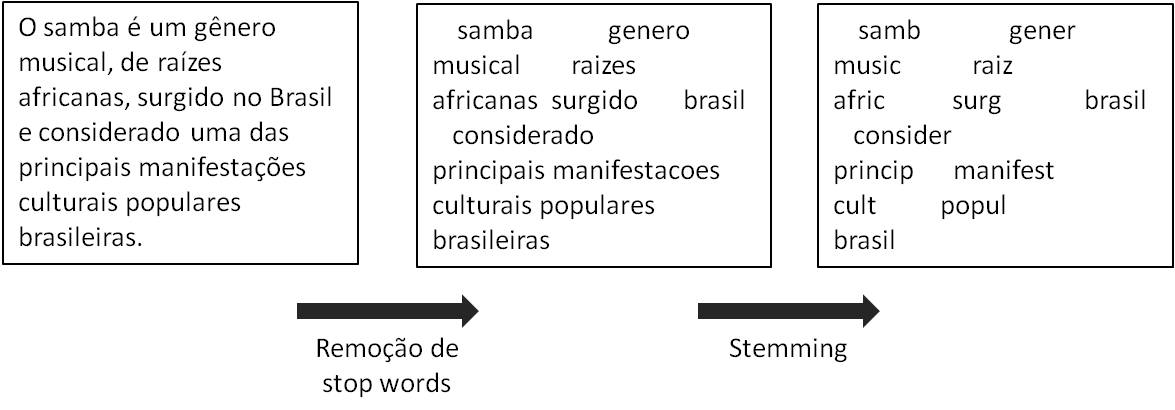
\includegraphics[width=0.45\textwidth]{exemplo-preprocessamento.jpg}
%	\caption{Exemplo de pré-processamento.}
%	\label{fig:exemplopreprocessamento}
%  \end{figure}






\subsection{Identificação de candidatos}
	\label{subsec:indentificacaosentencas}
	
%%%%%%%%%%	
% Indicar unidade mínima de Segmento
%%%%%%%%%%
	
	
%	Como entrada para os 
%	Os algoritmos de segmentação devem ser
	É preciso fornecer aos algoritmos os candidatos iniciais a limites de segmento. Para isso, é necessário escolher qual será a unidade de informação mínima que constitui um segmento. Baseando-se no estilo de escrita e considerando as pontuações de um texto, é possível, em alguns casos, indicar quebras de parágrafo, finais de sentenças ou mesmo palavras como elementos que encerram um segmento. 

	Ocorre que em atas de reunião é uma prática comum redigi-las de forma que o conteúdo discutido fica em parágrafo único, além disso, as quebras de parágrafo são usados para formatação de outros elementos como espaço para assinaturas. 
%
	Também não é conveniente indicar todo ponto entre \textit{token} como candidato pois obrigaria a ajustar posteriormente os segmentos de maneira a não quebrar uma ideia ou frase. 
%	
	Assim, neste trabalho, os finais de sentença são considerados unidades de informação e portanto, passíveis a limite entre segmentos. 
	
	Devido ao estilo de pontuação desses documentos, como encerrar sentenças usando um \textit{";"} e inserção de linhas extras, foram usadas as regras apresentadas no Algoritmo 1 para identificar os finais de sentenças.  


\begin{algorithm}
	\SetKwInOut{Input}{Entrada}
	\SetKwInOut{Output}{Saída}
	\SetKwBlock{Inicio}{início}{fim}
	\SetKwFor{ParaTodo}{para todo}{}{fim para todo}
	\SetKwIF{Se}{SenaoSe}{Senao}{}{}{senao se}{senao}{fim se}
	\SetKwFor{Para}{}{}{}
%	\SetKwAlgorithm{Algorithm}{Algoritmo}{}

	
	\Input{Texto}
	\Output{Texto com identificações de finais de sentença}
	
	\ParaTodo {token, marcá-lo como final de sentença se:} {	

	Terminar com um \texttt{!}\\
	Terminar com um \texttt{.} e não for uma abreviação\\
	Terminar em \texttt{.?;} e:
		\Para{}{
			For seguido de uma quebra de parágrafo ou tabulação\\
			O próximo \textit{token} iniciar com  \texttt{(\{["'}\\
			O próximo \textit{token} iniciar com letra maiúscula\\
			O penúltimo caracter  for \texttt{)\}]"'}\\
		}
	}
	
	\caption{Identificação de finais de sentença}
	\label{alg:identificacaofinaisdesent}
\end{algorithm}









%Como forma de padronização, as instituições acrescentam ao documento

%		passos menores
%		1 - heurística simples para remover cabeçalho e rodapé.
%		2 - remoção de numerais
%		3 - remoção de acentos, transformações de caixa, remoção de pontuação.
		
	% Esses passos são realizados internamente em cada algorímo, para que a saida seja legível ao usuário final.





%A qualidade do algoritmo é sempre dependente da escrita correta! Ausência de emoticons, códigos de computador e gírias.





%Nas subseções a seguir serão expostas as alterações para aumentar a eficiência dos algoritmos e encontrar o melhor modelo para a tarefa de segmentar o texto das atas em tópicos.



%Tais aspectos não se aplicam ao contexto das atas, onde o estilo de escrita em forma de narrativa, prefere poupar o leitor de diálogos secundários durante transições de tópicos. 







	
	
%Elimina-se textos considerados de pouca relevância como a numeração de páginas e linhas, cabeçalhos e rodapés, também elemina-se acentuação, sinais de pontuação, restando apenas palavras.  


	
	
%%
%% 1) Identificação de sentenças
%Primeiro cada final de sentença e identificado e marcado com uma \textit{string} especial, esse processo é melhor descrito na Subseção~\ref{subsec:indentificacaosentencas}.
%%
%%conforme mostrado no Algoritmo~\ref{alg:identificacaofinaisdesent}.
%
%%	
%% 2) Eliminação de ruídos
%Depois, elimina-se textos considerados de pouca relevância como a numeração de páginas e linhas, cabeçalhos e rodapés, também elemina-se acentuação, sinais de pontuação, restando apenas palavras.  
%
%%	
%% 3) Stop Words
%Em seguida, remove-se as palavras consideradas menos informativas, as quais são chamadas de \textit{stop words}, para isso, utiliza-se uma lista contendo 438 palavras. 
%
%%
%% 4) Stemming
%Por fim, extrai-se o radical de cada palavra, para isso, as letras são convertidas em caixa baixa e aplica-se o algoritmo \textit{Orengo}\footnote{\urlorengo} para remoção de sufixos.
%
%
%Tem-se então, uma lista com os elementos considerados mais significativos do texto. A Figura~\ref{fig:exemplopreprocessamento} mostra a etapa de pré-processamento em uma sentença em português.
%	





	
	
\section{Avaliação}
	\label{sec:avaliacao}



%%%%%%%%%% 
% Necessidade de uma referência
%%%%%%%%%%
Para que se possa avaliar um segmentador automático de textos, é preciso uma referência, isto é, um texto com os limites entre os segmento conhecidos. Essa referência, deve ser confiável, sendo uma segmentação legítima que é capaz de dividir o texto em porções relativamente independentes, mantendo um conteúdo legível, ou seja, uma segmentação ideal.
%

Entre as abordagens mais comuns para se conseguir essas referências, encontramos: A concatenação aleatória de documentos distintos, onde o ponto entre o final de um texto e o inicio do seguinte é um limite entre eles. A segmentação manual dos documentos, nesse caso, pessoas capacitadas, também chamadas de juízes, ou mesmo o autor do texto, são consultadas e indicam manualmente onde há uma quebra de segmento. Em transcrição de conversas faladas em reuniões com múltiplos participantes, um mediador é responsável por encerrar um assunto e iniciar um novo, nesse caso o mediador anota manualmente o tempo onde há uma transição de tópico. Em aplicações onde a segmentação é tarefa secundária, analisar seu impacto na aplicação final.


%%%%%%%%%%
% As 2 principais dificuldades na avaliação
%%%%%%%%%%
De acordo com \cite{Pevzner2002} há duas principais dificuldades na avaliação de segmentadores automáticos. A primeira é conseguir um referência, já que juízes humanos costumam não concordar entre si, sobre onde os limites estão e outras abordagens podem não se aplicar ao contexto. A segunda é que tipos diferentes de erros devem ter pesos diferentes de acordo com a aplicação. Há casos onde certa imprecisão é tolerável e outras, como a segmentação de notícias, onde a precisão é mais importante.


%%%%%%%%%%
% Definição do que é um bom algoritmo de segmentação
%%%%%%%%%%
Para fins de avaliação desse trabalho, um bom método de segmentação é aquele cujo resultado melhor se aproxima do ideal, sem a obrigatoriedade de estar perfeitamente alinhado com tal. Ou seja, visto o contexto das atas de reunião, e a subjetividade da tarefa, não é necessário que os limites entre os segmentos (real e hipótese) sejam idênticos, mas que se assemelhem em localização e quantidade.


Para quantificar a eficiência dos algoritmos, segue uma revisão das principais métricas aplicáveis.

As próximas subseções mostram o conjunto de atas e a segmentação usada como referência, uma revisão das principais métricas aplicáveis à segmentação e os testes realizados a fim de avaliar os métodos

\subsection{Conjunto de documentos}
	A fim de obter um conjunto de documentos segmentados que possam servir como referência na avaliação, seis atas de reunião foram coletadas junto ao departamento de computação da UFSCar-Sorocaba. Os documentos foram oferecidos à profissionais que participam de reuniões desse departamento e por meio de um \textit{software} segmentaram o texto das atas conforme o julgamento de cada um. Os segmentos gerados manualmente foram comparados à segmentação automática conforme os critérios descritos a seguir.
	
	As atas de reunião diferem dos textos comumente estudados em outros trabalho em alguns pontos.
	


\subsection{Medidas de Avaliação}


	As medidas de avaliação tradicionalmente utilizadas em \textit{information retrieval} como precisão e revocação trazem alguns problemas na avalização de segmentadores automáticos.  
Conforme o algoritmo aponta mais segmentos no texto, tende a melhorar a revocação e ao mesmo tempo, reduzir a precisão, um problema que pode ser contornado usando \textit{F-measure} que faz uma combinação da duas levando em conta seus pesos, o que por outro lado é mais difícil de interpretar. 
Essas medidas falham ao não serem sensíveis a \textit{near misses}, ou seja, quando um limite não coincide exatamente com o esperado, mas fica próximo~\cite{Kern2009}.

A Figura~\ref{fig:exemplosegmentacaozoom} mostra um exemplo com duas segmentações hipotéticas e uma referência. Em ambos os casos não há nenhum verdadeiro positivo, o que implica em zero para os valores de precisão, acurácia, e revocação, embora a segunda hipótese possa ser considerada superior à primeira se levado em conta a proximidade dos limites.



  \begin{figure}[!h]

	\centering
	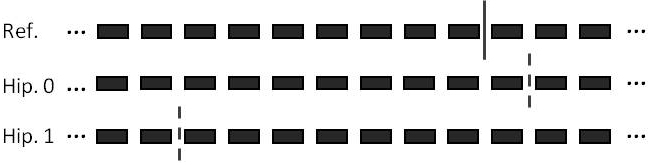
\includegraphics[width=0.47\textwidth]{windiffzoom.jpg}
	\caption{Exmplos de segmentação}
	\label{fig:exemplosegmentacaozoom}

  \end{figure}



\subsubsection{P$_k$}
A fim de resolver o problema de \textit{near misses}, Beeferman \textit{et. al.}~\cite{Beeferman1999} apresentam uma nova medida chama P$_k$ que atribui valores parciais a \textit{near misses}. Esse método move uma janela de tamanho $k$ e a cada posição e verifica se o início e o final da janela estão ou não dentro do mesmo segmento e penaliza o algoritmo em caso de discrepância. 

Ou seja, dado duas palavras de distancia $k$, uma discrepância é computada quando o algoritmo e a referência não concordam se as palavras estão ou não no mesmo segmento.

O valor de $k$ é calculado como a metade da média dos comprimentos dos segmentos reais. Como resultado, é retornado a contagem de discrepâncias divido pelo quantidade de segmentações analisadas. Esse valor serve como medida de dissimilaridade entre as segmentações e pode ser interpretada como a probabilidade de duas sentenças extraídas aleatoriamente pertencerem ao mesmo segmento.



\subsubsection{WindowDiff}

Pevzner~\cite{Pevzner2002} aponta problemas na avaliação mais tradicional Pk~\cite{Beeferman1999}. Eles apontam que esse método penaliza demasiadamente os falsos negativos em relação aos falsos positivos e a \textit{near misses}, além disso, desconsidera o tamanho e a quantidade de segmentos, entre outros problemas.

Como solução, propõem um novo método, o qual chamam de \textit{WindowDiff} que traz duas diferenças principais: a dobra a penalidade para os falsos positivos a fim de diminuir o problema da subestimação dessa medida e, diferente de P$_k$, ao mover a janela pelo texto, penaliza o algoritmo sempre que o número de limites proposto pelo algoritmo não coincidir com o número de limites esperados para aquela janela de texto. 

Com isso, demonstram em seu trabalho que, em relação a P$_k$, consegue resolver seus principais problemas e mantém sua proposta inicial de sensibilidade a \textit{near misses}, penalizando-os menos que os falsos positivos puros.


  \begin{figure}[!h]

	\centering
	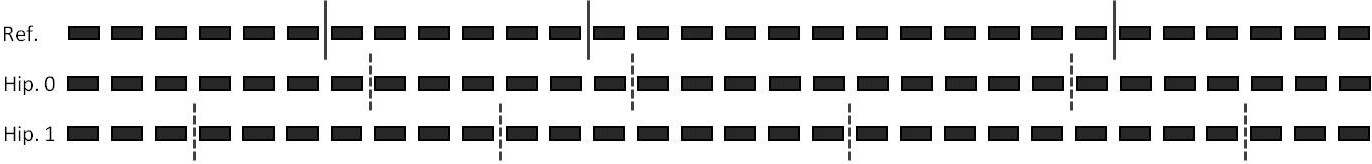
\includegraphics[width=0.47\textwidth]{windiff.jpg}
	\caption{Exemplo de construção de uma matriz de rank}
	\label{fig:exemplosegmentacao}

  \end{figure}
  
  

%Falar do software para segmentação manual????


\subsection{Avaliação dos segmentadores}


%%%%%%%%%%
% Parâmetros
%%%%%%%%%%
As implementações dos algoritmos permitem ao usuário a configuração de seus parâmetros. 
%
O \textit{TextTiling} permite ajustarmos dois parâmetros, sendo, o tamanho da janela (distância entre a primeira e a última sentença) para o qual atribuiu-se os valores 20, 40 e 60. O segundo parâmetro, o passo (distância que a janela desliza), atribuiu-se os valores 3, 6, 9 e 12. Gerando ao final 18 modelos.
%

O \textit{C99} permite ajustarmos três parâmetros, sendo, a quantidade segmentos desejados, o qual é calculado como uma proporção dos candidatos a limite. Para isso atribuiu-se as proporções de 0,2 a 1,0 em intervalos de 0,2 O segundo parâmetro, o tamanho da máscara utilizada para gerar a matriz de ranking, atribuiu-se os valores 9 e 11. Permite ainda, definirmos se as sentenças serão representados por vetores contendo a frequência ou o peso de cada termo, onde ambas as representações foram utilizadas. Gerando ao final 20 modelos.



%%%%%%%%%%
% Cálculo das medidas para cada modelo
%%%%%%%%%%
Pela comparação dos resultados com a segmentação fornecida pelos especialistas, calculou-se para cada modelo as medidas tradicionais acurácia, precisão, revocação, F-medida. Além dessas, computou-se também as métricas mais aplicadas à segmentação textual P$_k$ e \textit{WindowDiff}.



%%%%%%%%%%
% Teste de Fiedman e CD
% 1ª Etapa
%%%%%%%%%%
Em seguida aplicou-se o teste de Friedman a fim de saber se há diferenças significativas entre a eficácia dos modelos, o pós-teste de Nemenyi foi aplicado para descobrir quais diferenças são significativas. 
%
Exite diferença quando seus \textit{rankings} médios diferirem em um valor mínimo, chamado de diferença critica (CD). 
%

%%%%%%%%%%
% Dados Obtidos
%%%%%%%%%%
Com isso foi possível, pela análise do diagrama de diferença crítica, verificar qual é o melhor modelo para cada medida
% e quão significativamente 
em relação aos demais. 


A tabela~\ref{tab:mediasC99} mostra os dados obtidos com o \textit{C99}, onde \texttt{S} é a proporção de segmentos em relação a quantidade de candidatos, \texttt{M} é o tamanho da máscara utilizada para criar a matriz de \textit{ranking} e \texttt{W} indica se os segmentos são representados por vetores contendo a frequência ou um peso das palavras. 



\begin{table}[!h]
	\centering

	\begin{tabular}{|c|c|c|c|c|}
	
		\hline
		Medida & \texttt{S} & \texttt{M} & \texttt{W} & \textbf{Média}\\		
		\hline

		Acuracy		& 40	& 11 & Sim & 0.6199	\\ \hline	
		F1			& 60	& 9	 & Sim & 0.6167	\\ \hline	
		Precision	& 40	& 11 & Sim & 0.7106	\\ \hline			
		Recall		& 100	& 9	 & Não & 0.8516	\\ \hline		
		Pk			& 40	& 11 & Sim & 0.1163	\\ \hline	
		Windiff		& 40	& 11 & Sim & 0.3800	\\ \hline		

		
	\end{tabular}
	
	\caption{Médias das medidas obtidas com \textit{C99}}
	\label{tab:mediasC99}
\end{table}


A tabelas~\ref{tab:mediasTextTiling} mostra os dados obtidos com o \textit{TextTiling}, \texttt{J} é o tamanho da janela e \texttt{P} e o passo.

\begin{table}[!h]
	\centering

	\begin{tabular}{|c|c|c|c|}
	
		\hline
		Medida & \texttt{J} & \texttt{P} & \textbf{Média}\\		
		\hline

		Acuracy		& 50 & 9 	& 0.5510 \\ \hline	
		F1			& 50 & 3 	& 0.5898 \\ \hline	
		Precision	& 60 & 12 	& 0.5746 \\ \hline			
		Recall		& 50 & 3 	& 0.7717 \\ \hline		
		Pk			& 30 & 9 	& 0.1572 \\ \hline	
		Windiff		& 50 & 9 	& 0.4489 \\ \hline		

		
	\end{tabular}
	
	\caption{Médias das medidas obtidas com o \textit{TextTiling}}
	\label{tab:mediasTextTiling}
\end{table}


Uma vez sabendo quais valores de parâmetros melhor configuram um algoritmo para uma medida, resta então saber qual dos dois algoritmos é mais eficiente segundo essa medida. Para isso aplicou-se novamente o teste de Friedman com pós-teste de Nemenyi, dessa vez, com os melhores modelos dos dois algoritmos para cada medida. O resultado segue na Tabela~\ref{tab:melhoresmodelos}

\begin{table}[!h]
	\centering
	
	\begin{tabular}{|c|c|c|c|c|}

		\hline
		Medida & Algoritmo & \texttt{S} & \texttt{M} & \texttt{W}\\		
		\hline
		
	
		Acuracy		& C99 & 40 	& 11	& Sim \\ \hline
		Precision	& C99 & 40 	& 11	& Sim \\ \hline
		Pk			& C99 & 40 	& 11	& Sim \\ \hline
		Windiff		& C99 & 40 	& 11	& Sim \\ \hline
		F1			& C99 & 60 	& 9		& Sim \\ \hline
		Recall		& C99 & 100 & 9		& Não \\ \hline
 	
	
	\end{tabular}

	\caption{Melhores modelos para cada medida segundo diagramas de diferença crítica}
	\label{tab:melhoresmodelos}	
	
\end{table}


Na análise do diagrama de diferença crítica verificou-se que o algoritmo \textit{C99} apresenta melhor eficiência em todas as medidas e os valores das quatro primeiras os valores de \texttt{S}, \texttt{M} e \texttt{W} se repetiram, sugerindo uma configuração otimizada para o problema da segmentação de atas de reunião.







	\section{Resultados}
	\label{sec:resultados}

%%%%%%%%%%
% Objetivos
%%%%%%%%%%
A fim de encontrar o melhor método que divida uma ata em segmentos coerentes, realizou-se experimentos com o \textit{TextTiling} e \textit{C99} a fim de encontrar os melhores parâmetros para esses documentos.

%tópicos retornando segmentos  que retorne segmentos coerentes 

%%%%%%%%%%
% Parâmetros
%%%%%%%%%%
As implementações dos algoritmos permitem ao usuário a configuração de seus parâmetros. 
%
O \textit{TextTiling} permite ajustarmos dois parâmetros, sendo, o tamanho da janela (distância entre a primeira e a última sentença) para o qual atribuiu-se os valores 20, 40 e 60. Para o segundo parâmetro, o passo (distância que a janela desliza), atribuiu-se os valores 3, 6, 9 e 12. Gerando ao final 20 modelos.
%

O \textit{C99} permite ajustarmos três parâmetros, sendo, a quantidade segmentos desejados, o qual é calculado como uma proporção dos candidatos a limite. Para isso atribuiu-se as proporções {0,2; 0,4; 0,6; 0,8; 1,0}. O segundo parâmetro, o tamanho da máscara utilizada para gerar a matriz de ranking, atribuiu-se os valores 9 e 11. Permite ainda, definirmos se as sentenças serão representados por vetores contendo a frequência ou o peso de cada termo, onde ambas as representações foram utilizadas.
%
 Considerando todos os parâmetros, foram gerados 20 modelos para o algoritmo C99.% By Rafael 



%%%%%%%%%%
% Cálculo das medidas para cada modelo
%%%%%%%%%%

% --> Isso já foi falado no texto
%Pela comparação dos resultados com a segmentação fornecida pelos especialistas, calculou-se para cada modelo as medidas tradicionais acurácia, precisão, revocação, F-medida. Além dessas, computou-se também as métricas mais aplicadas à segmentação textual P$_k$ e \textit{WindowDiff}.



%%%%%%%%%%
% Teste de Fiedman e CD
% 1ª Etapa
%%%%%%%%%%
Em seguida aplicou-se o teste de Friedman a fim de saber se há diferenças significativas entre a eficácia dos modelos. O pós-teste de Nemenyi foi aplicado para descobrir quais diferenças são significativas. 
%
Exite diferença quando seus \textit{rankings} médios diferirem em um valor mínimo, chamado de diferença critica (CD). 
%

%%%%%%%%%%
% Dados Obtidos
%%%%%%%%%%
Com isso foi possível, pela análise do diagrama de diferença crítica, verificar qual é o melhor modelo para cada medida
% e quão significativamente 
em relação aos demais. 


A Tabela~\ref{tab:mediasC99} mostra os dados obtidos com o \textit{C99}, onde \texttt{S} é a proporção de segmentos em relação a quantidade de candidatos, \texttt{M} é o tamanho da máscara utilizada para criar a matriz de \textit{ranking} e \texttt{W} indica se os segmentos são representados por vetores contendo a frequência ou um peso das palavras. 



\begin{table}[!h]
	\centering

	\begin{tabular}{|c|c|c|c|c|}
	
		\hline
		Medida & \texttt{S} & \texttt{M} & \texttt{W} & \textbf{Média}\\		
		\hline

		Acuracy		& 40	& 11 & Sim & 0.6199	\\ \hline	
		F1			& 60	& 9	 & Sim & 0.6167	\\ \hline	
		Precision	& 40	& 11 & Sim & 0.7106	\\ \hline			
		Recall		& 100	& 9	 & Não & 0.8516	\\ \hline		
		Pk			& 40	& 11 & Sim & 0.1163	\\ \hline	
		Windiff		& 40	& 11 & Sim & 0.3800	\\ \hline		

		
	\end{tabular}
	
	\caption{Médias das medidas obtidas com \textit{C99}}
	\label{tab:mediasC99}
\end{table}


A tabelas~\ref{tab:mediasTextTiling} mostra os dados obtidos com o \textit{TextTiling}, onde \texttt{J} é o tamanho da janela e \texttt{P} é o passo.

\begin{table}[!h]
	\centering

	\begin{tabular}{|c|c|c|c|}
	
		\hline
		Medida & \texttt{J} & \texttt{P} & \textbf{Média}\\		
		\hline

		Acuracy		& 50 & 9 	& 0.5510 \\ \hline	
		F1			& 50 & 3 	& 0.5898 \\ \hline	
		Precision	& 60 & 12 	& 0.5746 \\ \hline			
		Recall		& 50 & 3 	& 0.7717 \\ \hline		
		Pk			& 30 & 9 	& 0.1572 \\ \hline	
		Windiff		& 50 & 9 	& 0.4489 \\ \hline		

		
	\end{tabular}
	
	\caption{Médias das medidas obtidas com o \textit{TextTiling}.}
	\label{tab:mediasTextTiling}
\end{table}


Uma vez sabendo quais valores de parâmetros melhor configuram um algoritmo para uma medida, resta então saber qual dos dois algoritmos é mais eficiente segundo essa medida. Para isso aplicou-se novamente o teste de Friedman com pós-teste de Nemenyi, dessa vez, com os melhores modelos dos dois algoritmos para cada medida. O resultado segue na Tabela~\ref{tab:melhoresmodelos}

\begin{table}[!h]
	\centering
	
	\begin{tabular}{|c|c|c|c|c|}

		\hline
		Medida & Algoritmo & \texttt{S} & \texttt{M} & \texttt{W}\\		
		\hline
		
	
		Acuracy		& C99 & 40 	& 11	& Sim \\ \hline
		Precision	& C99 & 40 	& 11	& Sim \\ \hline
		Pk			& C99 & 40 	& 11	& Sim \\ \hline
		Windiff		& C99 & 40 	& 11	& Sim \\ \hline
		F1			& C99 & 60 	& 9		& Sim \\ \hline
		Recall		& C99 & 100 & 9		& Não \\ \hline
 	
	
	\end{tabular}

	\caption{Melhores modelos para cada medida segundo diagramas de diferença crítica.}
	\label{tab:melhoresmodelos}	
	
\end{table}


Na análise do diagrama de diferença crítica verificou-se que o algoritmo \textit{C99} apresenta melhor eficiência em todas as medidas e os valores das quatro primeiras os valores de \texttt{S}, \texttt{M} e \texttt{W} se repetiram, sugerindo uma configuração otimizada para o problema da segmentação de atas de reunião.






	\section{Conclus�o}
	\label{sec:conclusao}

As atas de reuni�o, objeto de estudo desse artigo, apresentam caracter�sticas peculiares em rela��o � discursos e textos em geral. Caracter�sticas como segmentos curtos e coes�o mais fraca devida ao estilo que evita repeti��o de palavras e ideias em benef�cio da leitura por humanos, dificultam o processamento por computadores.

%%%%%%%%%%
% Benef�cios 
%%%%%%%%%%


Os algoritmos \textit{TextTiling} e \textit{C99} foram testados em um conjunto de atas coletadas do Departamento de Computa��o da UFSCar-Sorocaba. Por meio da an�lise dos dados chegou-se a uma configura��o cujos segmentos melhor se aproximaram das amostras segmentadas por participantes das reuni�es. 


Na maioria das medidas, o algoritmo \textit{C99} sobressaiu-se em rela��o ao \textit{TextTiling}, contudo, os testes estat�sticos, n�o apresentam diferen�a significativa. 


%%%%%%%%%%%%%%%
% O Impacto do Preprocessamento 
%%%%%%%%%%%%%%%

Da mesma forma, a etapa de preprocessamento proporciona melhora de performance quando aplicada, por�m o seu maior benef�cio � a diminui��o do custo computacional, uma vez que n�o prejudica a qualidade dos resultados.



A segmenta��o de atas de reuni�o pode ajudar na organiza��o, busca e compreens�o dos conte�dos nelas contidos. Tamb�m outros dom�nios e aplica��es diferentes podem se beneficiar dos resultados apresentados, como aplica��es voltadas a resgate de informa��o, sumariza��o e acessibilidade. Assim, espera-se que outros trabalhos possam aproveitar deste.
	
	
Em trabalhos futuros, ser�o investigadas t�cnicas de extra��o de t�picos para descrever os segmentos e com isso aprimorar o acesso ao conte�do das atas de reuni�o.






\bibliographystyle{abbrv}
\bibliography{bibs}  % sigproc.bib is the name of the Bibliography in this case

% that's all folks
\end{document}
